\documentclass{article}

\usepackage[margin=1in]{geometry}
\usepackage[table]{xcolor}
\usepackage{graphicx}
\usepackage{wrapfig}
\usepackage{titlesec}
\usepackage{titling}
\usepackage{setspace}

\titleformat{\section}
{\large\bfseries}
{Method \thesection}
{0em}
{: }[]

\renewcommand{\maketitle}{\hspace{-22px}  \textbf{{\theauthor} \\
ASEN5158 \\
\today \\
{\thetitle}} \titlerule}

\definecolor{lightgray}{gray}{0.8}

\begin{document}

  \title{Homework 3}
  \author{Connor Johnstone}

  \maketitle

  \vspace{20px}
  \textbf{Assignment:
    Summarize published options proposed for future spacecraft atmosphere design set points (or trade space) against historical vehicles in terms of total pressure, ppO2, ppCO2, inert gas makeup, humidity and any other parameters indicated.
  }

  \setstretch{1}

  \section{The Design Space}

  There are many factors that go into determining the design space of a human space exploration mission atmospheric mixture and system. It first helps to understand the design space in terms of the partial pressure of oxygen, which is the primary driver for the health of the astronauts under normal circumstances. Much research has been done on this subject and, as such, we can define a curve over total pressure and oxygen percentage at which the human body would process: a normal (sea level) amount of oxygen (normoxic), too little oxygen for long term missions (hypoxic), and too much oxygen for long term exposure (hyperoxic). 

  Right away we now have an upper and lower bound on a useful design space for human spaceflight missions, but there are a couple of other key factors to take into consideration. In particular, while partial oxygen pressure is the factor that is most relevant to human physiology, oxygen as a percentage of total atmospheric gas is the most relevant in the combustion of flammable materials. It is generally recommended that 30\% oxygen by volume is the point at which materials will combust more readily than they would in a typical atmospheric mixture. Therefore we can bound our design trade space a bit further by requiring that we don't go above 30\% oxygen by volume. However, it should be noted (and will be noted later) that it took the American space program a good many years to recognize the seriousness of the increased flammability problem, notably leading to the fiery disaster of Apollo 1.

  The final trade space bound that I'll mention in this report is the necessity of an EVA and the problems that poses for mobility and acclimatization. Generally, high pressure in an EVA suit comes at the detriment of productivity as it cause issues in mobility and dexterity (due to suit rigidity). However, lower suit pressures require acclimatization in order to prevent health issues associated with decompression sickness (the bends). This process is called pre-breathing and generally takes time, increasing over larger changes in pressure. We can further bound our trade space by defining a suit pressure and a maximum allowable pre-breathe time. However, it should be noted that there does exist other solutions, including exercise during pre-breath (currently employed on the ISS) and variable pressure space-suits that would allow for some productivity during acclimatization (currently employed by the russian EVA suits).
  
  \section{Exploration Atmosphere}

  These considerations have recently been taken into account and, as a result, NASA developed in 2012 (and later refined) an atmospheric mixture entitled ``Exploration Atmosphere'' to attempt to provide a cost-effective standard that will prevent flammability problems while still providing an easier acclimatization process for EVAs. The standard that was decided on is at 8.2 psia and 34\% oxygen by volume. Notably, this is a little high on the oxygen flammability side of the design space. It is also somewhat hypoxic in comparison to sea level atmospheric conditions, but still within the range of safe, non-hypoxic oxygen concentrations. This hypoxic nature is meant to provide an ease of acclimatization for EVA objectives, as well as reducing the cost of the oxygen necessary to bring on such a trip.

  It should also be noted, that the balance of the gas in the ``Exploration Atmosphere'' mixture will be Nitrogen. This is seen as a very typical gas balance (being used in all previous missions where the atmosphere was not pure oxygen) and is very similar to the mixture found on Earth. However, there are some other options, including Helium.

  \section{Historical Context}

  Briefly, I will discuss the various atmospheric mixtures used in previous human spaceflight missions.

  \subsection{Mercury, Gemini, Early Apollo}

  During the Mercury missions and all subsequent missions until the Apollo 1 fire, pure oxygen was used on board the American spaceflight missions, nominally at a pressure of about 5.5 psia. This drastically reduced weight and cost, as well as provided plenty of oxygen (being almost a bit hyperoxic) to the crew. However, after the Apollo 1 accident, this approach was deemed too dangerous to be used as a standard for future missions.

  \subsection{Later Apollo Missions}

  For the later Apollo missions, they stopped using pure oxygen on the launch pad. Instead, they used a 40\% $O_2$ mixture on the launch pad, then cut that down to a pure oxygen atmosphere at 5 psi during the actual in-space portion of the flights. The LM (lunar module) was also at pure oxygen, although only at 4.8 psi. This setup accomodated the many EVAs that they performed quite nicely.

  \subsection{Russian Missions}

  The Russians, as far back as Salyut and Mir, have been using an atmospheric mixture at roughly sea level conditions. This has the advantage of being safer and easier for the cosmonauts who are used to breathing on the Earth, but comes at a financial and EVA-prebreathing cost.

  \subsection{SkyLab}

  With SkyLab we finally used an atmospheric profile that didn't involve pure oxygen. It was about 70\% oxygen at around the same 5 psi of previous missions such as Apollo. This resolved some of the flammability concerns as well as not being as hyperoxic as the pure oxygen environment. In fact, it was nearly a sea-level equivalent mixture.

  \subsection{Shuttle, ISS, and Mir}

  All of our recent missions into space have been for longer term objectives, with increased risk of fire or health problems, since the astronauts are on board for weeks or months at a time. Therefore, we simply use atmospheric air mixtures and spend increased time in pre-breathe before EVAs.

  The chart and table on the next page place all of these historical context for easy reference:

  \begin{figure}[h!]
    \begin{center}
      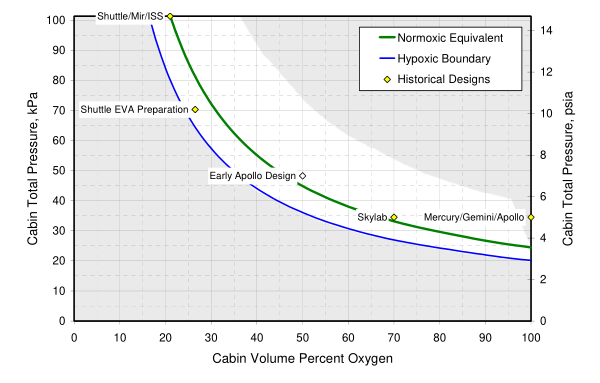
\includegraphics[width=0.95\linewidth]{historic_reference.png}
      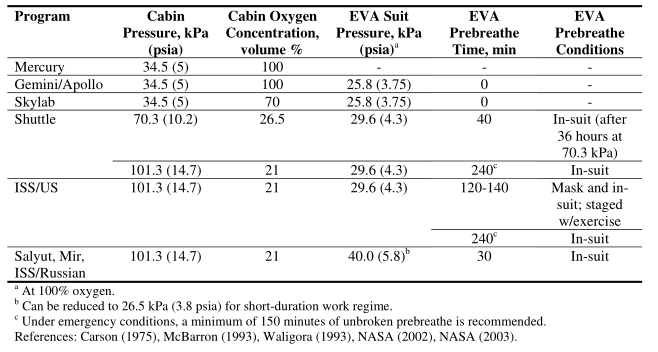
\includegraphics[width=0.95\linewidth]{table.png}
    \end{center}
  \end{figure}


\begin{thebibliography}{9}

  \bibitem{lange}
    Kevin Lange, Alan T. Perka, Bruce Duffield, Frank F. Jeng,
    \textit{Bounding the Spacecraft Atmosphere Design Space for Future Exploration Missions},
    NASA Johnson Space Flight Center,
    2005.

  \bibitem{abercromby}
    Andrew Abercromby, Johnny Conkin, Michael Gernhardt,
    \textit{Modeling a 15-min extravehicular activity prebreathe protocol using NASA's exploration atmosphere},
    Acta Astronautica,
    2015.

  \bibitem{norcross}
    Jason Norcross, Johnny Conkin, Grace Douglas,
    \textit{Risk of Hypoxia from the Exploration Atmosphere 1 Evidence Report: Risk of Hypobaric Hypoxia from the Exploration Atmosphere},
    NASA Johnson Space Flight Center,
    2015.

\end{thebibliography}

\end{document}
